\section{Organisation et Méthode}

\subsection{Rappel}

\begin{frame}{Rétrospective}
  \begin{block}{}
    \begin{itemize}
      \item Scrum
        \begin{itemize}
          \item Daily \emph{Scrum} (Meeting $\sim$2h30)
          \item \emph{Sprint}
        \end{itemize}
      \item EXtreme Programming
        \begin{itemize}
          \item Pair-programming
          \item Pair-Review + Dir. Technique Review
          \item Roulement des binômes
          \item Conventions de code
          \item Refactoring
        \end{itemize}
      \item Itérations avec le client
   \end{itemize}
  \end{block}
\end{frame}

\subsection{Que reste t-il de ces methodes?}

\begin{frame}{Scrum}
  \begin{block}{Que reste t-il de Scrum?}
    \begin{enumerate}
      \item Daily meeting concis ($\sim$30 min max)
        \begin{itemize}
          \item Rétrospective de la semaine
          \item (Ré)assignation des taches
        \end{itemize}
      \item \emph{Sprint} soutenu (tous ensemble vers l'objectif)
      \item Communication omni-présente au sein de l'équipe
    \end{enumerate}
  \end{block}
\end{frame}

\begin{frame}{EXtreme Programming}
  \begin{alertblock}{Que reste t-il de XP?}
    \begin{center}
      RIEN
      \begin{figure}
        
\includegraphics[scale=0.7]{img/coding_horror.png}
      \end{figure}
    \end{center}
    \end{alertblock}
\end{frame}


\subsection{FSF-XP et Objectif}

{
\usebackgroundtemplate{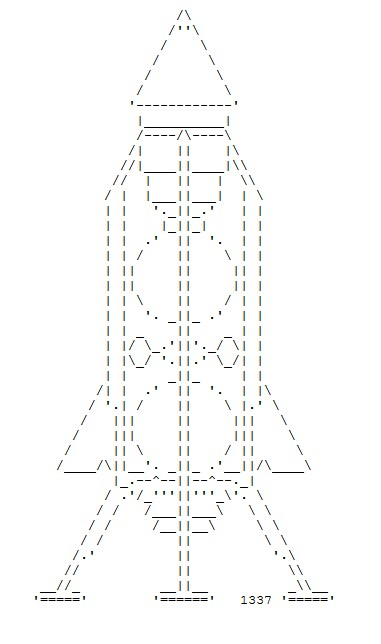
\includegraphics[scale=0.42]{img/rocket.jpg}}%
\begin{frame}{F-Safe Extreme Programming}
  \begin{exampleblock}{FSF-XP}
    \begin{itemize}
    \item ((bi|tri)nôme|petit-groupe)
    \item si un sous-groupe fonctionne, il se stabilise sinon il y a roulement
    \item review sur rétro-projecteur du code avec toute l'équipe
    \item Sprint avant livraison
    \end{itemize}
  \end{exampleblock}
\end{frame}
}

\begin{frame}{FSF-XP Sprint}
  \begin{itemize}
  \item Début de séance : On note les tâches et les propriétaires au tableau
  \item On définit les tâches à réaliser avant manger (\emph{manger blocker})
  \item Lorsque un groupe finit une tâche, on applaudit et on réassigne
  \end{itemize}
\end{frame}


\begin{frame}{FSF-XP Sprint}
  \begin{block}{}
    ``[...]it takes you a while to get into it and it takes 
    you a while to get back and remember where you were[...]''\footnote{G.Mark C.S Dep California}
  \end{block}
  \begin{block}{la bulle}
    \begin{itemize}
    \item on met en place les bulles (avec ou sans fenêtre)
    \item un consultant qui consulte les bulles et réponds aux questions diverses
    \end{itemize}
  \end{block}
\end{frame}


\begin{frame}{Déroulement d'une séance}
  \begin{figure}
    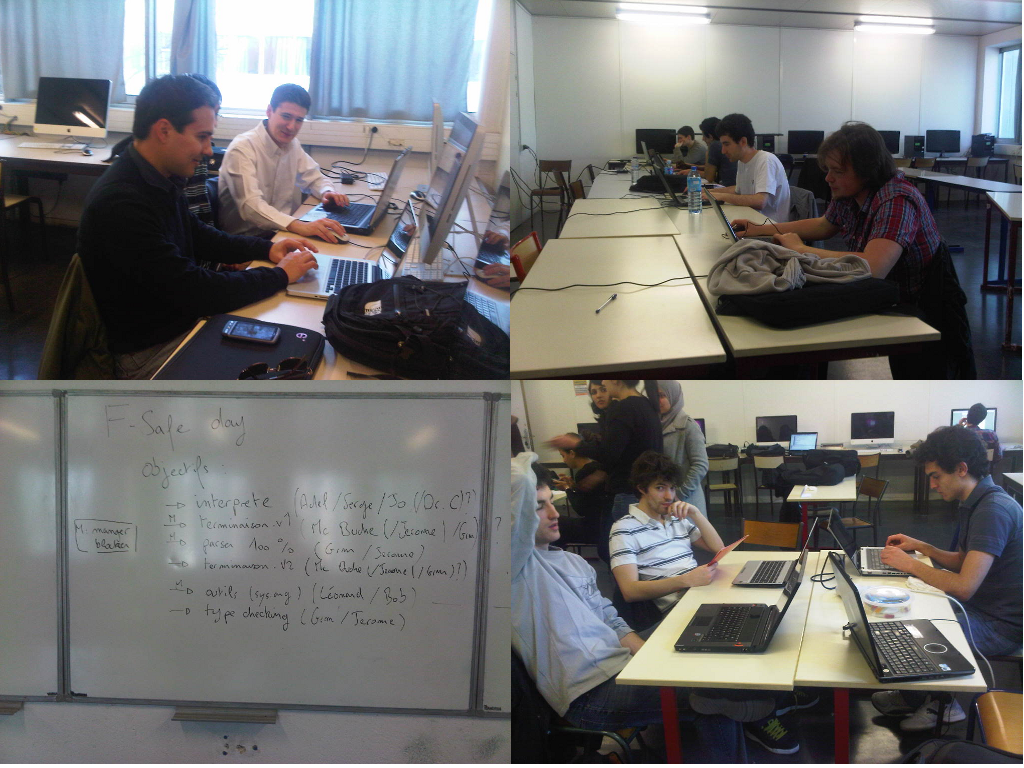
\includegraphics[scale=0.27]{img/FSafeDay.png}
  \end{figure} 
\end{frame}

\begin{frame}{Le travail à distance à 11}
  \begin{block}{}
    \begin{itemize}
      \item Push! Push! Push!
      \item création d'un document de suivi: Task, Status, Comment: \{Owner, Technical Dir.\}
      \item le directeur technique est le seul à fermer la \emph{RC} pour la demo client
    \end{itemize}
  \end{block}
\end{frame}


\subsection{Faisons un point...}

\begin{frame}{Calendrier}
  \begin{itemize}
    \item implémentation (cycle régulier) 
    \item sprint 1, 9/10 Mars
    \item démo client, 12 Mars => \emph{Objectif OK!}
    \item sprint 2, 14/15 Mars
    \item Release Candidate 18 Mars => \emph{Objectif OK!}
    \item stabilisation de la Release
    \item livraison, 21 Mars
  \end{itemize}
\end{frame}


